\newpage
\chapter{Berechnung der Schnittkräfte}
\section{Berechnung der auf die Zahnräder wirkenden Kräfte}

Da im Gang 2 das höchste Moment auf die Welle I wirkt, wird auch für diesen Gang der Schnittkräfteverlauf berechnet. Hierfür muss zuerst berechnet werden, welches Moment auf das jeweilige Zahnrad wirkt. Hierfür wird die folgende Beziehung genutzt:
\[M = \frac{P}{2\pi \x n_c}\] 
Als Leistung wird hierbei die jeweils übertragene Leistung angenommen, d.h. auf Zahnrad 8 wirkt die Schnittleistung (die Leistung der Welle II) und auf Zahnrad 6 die Leistung der Welle IV.
	\begin{align*}
M_8 &= \frac{P_c}{2\pi \x n_{an}} = \frac{7466,91 \text { W}}{2\pi \x 1200 \frac{1}{60 \text{ s}}}= 59,42 \text{ Nm}\\
M_6 &= \frac{P\textsubscript{IV,2}}{2\pi \x n_{an}} = \frac{94,31 \text{ W}}{2\pi \x 1200 \frac{1}{60 \text{s}}}= 0,75 \text{ Nm}\\
\end{align*}
\begin{center}
	\textbf{Stirnrad 6} \\
	\vspace{.5cm}
	Gegebene Werte: $M\textsubscript{6} = 0,75 \text{ Nm}, \qquad \alpha = 20^\circ, \qquad d_6 =178 \text{ mm}$
	\begin{align*}
	F\textsubscript{t,6} &= \frac{2\x M\textsubscript{6}}{d_6} = \frac{2 \x 0,75 \text{ Nm}}{0,178 \text{ m}} = 8,43 \text{ N}\\ 
	F\textsubscript{r,6} &= F\textsubscript{t,6} \x \tan{\alpha} =8,43 \text{ N} \x \tan{(20^\circ)} = 3,07 \text{ N}\\ 
	F\textsubscript{a,6} &= 0\text{ N}\\
	\end{align*}
	\newpage
	\textbf{Kegelrad 8}\\
	\vspace{.5cm}
	Formel aus Roloff/Matek\ccite{bib:roloffMatek:maschinenelemente} Seite 795 \\
	\vspace{.3cm}
	Gegebene Werte: $M\textsubscript{8} = 59,42 \text{ Nm}, \qquad \delta_8 = 36,13^\circ, \qquad d_8 = 124 \text{ mm}, \qquad \alpha = 20^\circ $
	\begin{align*}
	d\textsubscript{m,8} &= d_8 - b_8 \x \sin{\delta_8} = 124 \text{ mm} - 30\text{mm} \x \sin{(36,13^\circ)} = 106,31 \text{ mm}\\ 
	F\textsubscript{tm,8} &= \frac{2 \x M\textsubscript{8}}{d\textsubscript{m,8}} = \frac{2 \x 59,42 \text{ Nm} } {0,10631 \text{ m}} = 1117,86 \text{ N}\\
	F\textsubscript{r,8} &= F\textsubscript{tm,8} \x \tan{\alpha} \x \cos{\delta_8} = 328,62 \text{ N}\\ 
	F\textsubscript{a,8} &= F\textsubscript{tm,8}\x \tan{\alpha} \x \sin{\delta_8} = 239,9 \text{ N} \\ 
	\end{align*}
\end{center}
\newpage
\section{Berechnung der Lagerreaktionen}
\begin{center}
	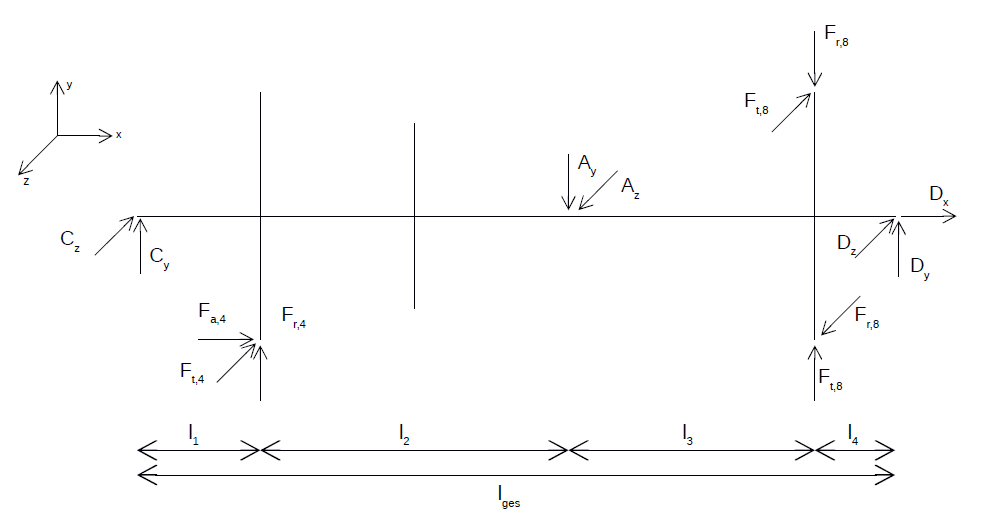
\includegraphics{figures/Uebersicht}
\end{center}
Gegebene Werte:
\[l_1 = 409\text{ mm} , \qquad l_2 = 60,7\text{ mm}, \qquad l_3 =366,5\text{ mm}, \qquad l\textsubscript{ges}= 808,2\text{ mm} , \qquad F_K=2318,49 \text{ N} \]
\begin{align*}
    \sum F_z &\overset{!}{=} 0 = A_z + F\textsubscript{a,8} - F_K \implies A_z = - F\textsubscript{a,8} + F_K = 2078,59 \text{ N}\\ 
    \sum F_y &\overset{!}{=} 0 = -A_y- B_y - F\textsubscript{t,6} + F\textsubscript{t,8}\\ 
    \sum F_x &\overset{!}{=} 0 = A_x + B_x - F\textsubscript{r,8} + F\textsubscript{r,6}\\ \\
    \sum M\textsubscript{y}\textsuperscript{(A)} &\overset{!}{=} 0 =  l_1 \x F\textsubscript{r,8} - (l_1+l_2) \x F\textsubscript{r,6}+ \frac{d\textsubscript{m,8} }{2}\x F\textsubscript{a,8}- l\textsubscript{ges} \x B_x\\ 
    &\implies B_x = \frac{F_{r,8} \x l_1 + F_{a,8}\x \frac{d_{m,8}}{2}-F_{r,6}\x (l_1 + l_2)}{l_{ges}} = 180,11 \text { N} \\ 
    & \implies A_x = F\textsubscript{r,8} - F\textsubscript{r,6} - B_x = 145,44 \text{ N}\\ \\
    \sum M\textsubscript{x}\textsuperscript{(A)} &\overset{!}{=} 0 = l\textsubscript{ges} \x B_y - l_1 \x F\textsubscript{t,8} + (l_1+l_2) \x F\textsubscript{t,6} \\ 
    &\implies B_y = \frac{l_1\x F\textsubscript{t,8} - (l_1+l_2) \x F\textsubscript{t,6}}{l\textsubscript{ges}} = 560,8 \text{ N}\\ 
    & \implies A_y =   F\textsubscript{t,8}-B_y- F\textsubscript{t,6} =  548,63\text{ N}\\ 
\end{align*}
\begin{align*}
    A_x &= \underline{145,44\text{ N}} & B_x= \underline{180,11\text{ N}}\\
    A_y &= \underline{548,63\text{ N}} & B_y= \underline{560,8\text{ N}}\\
    A_z &= \underline{2078,59\text{ N}}
\end{align*}
\section{Berechnung der Schnittkraftverläufe}
\renewcommand{\labelenumi}{\roman{enumi})}
\begin{enumerate}
\item Bereich I: $0 \leq z_1 \leq l_1$
\begin{center}
	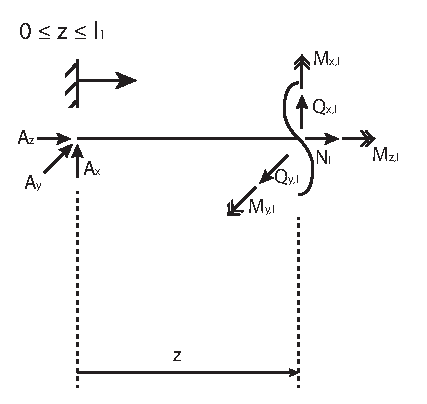
\includegraphics{figures/Bereich_1}
\end{center}
    \begin{align*}
        \sum F_x &\overset{!}{=} 0 = A_x + Q_{x,\mathrm{I}} \quad \implies \quad  Q_{x,\mathrm{I}} = -A_x = -145,44\text{ N}\\ 
        \sum F_y &\overset{!}{=} 0 =  Q_{y,\mathrm{I}} - A_y \quad \implies \quad  Q_{y,\mathrm{I}} = A_y = 548,63\text{ N}\\
        \sum F_z &\overset{!}{=} 0 = A_z + N_{\mathrm{I}} \quad \implies \quad  N_{\mathrm{I}} = -A_z = -2078,59\text{ N}\\
        \sum M_x \textsuperscript{(P)}&\overset{!}{=} 0 = M_{x,\mathrm{I}} - z \x A_y \quad \implies \quad   M_{x,\mathrm{I}} = z \x A_y = 548,63 \text{ N} \x z\\ 
        \sum M_y \textsuperscript{(P)}&\overset{!}{=} 0 = M_{y,\mathrm{I}} - z \x A_x \quad \implies \quad   M_{y,\mathrm{I}} = z \x A_x =154,44 \text{ N} \x z\\ 
        \sum M_z \textsuperscript{(P)}&\overset{!}{=} 0 = M_{z,\mathrm{I}}  \quad \implies \quad   M_{z,\mathrm{I}} = 0 \text{ N} \\ 
    \end{align*}
\newpage
\item Bereich II: $0 \leq z_2 \leq l_2$
\begin{center}
	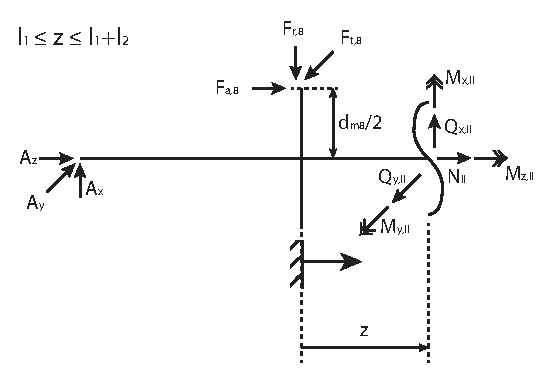
\includegraphics{figures/Bereich_2}
\end{center}
			\begin{align*}
        \sum F_x &\overset{!}{=} 0 = A_x -F\textsubscript{r,8} + Q_{x,\mathrm{II}} \\
				&\implies  Q_{x,\mathrm{II}} = F\textsubscript{r,8} -A_x =183,18 \text{ N}\\ \\
       \sum F_y &\overset{!}{=} 0 = -A_y +F\textsubscript{t,8} + Q_{y,\mathrm{II}} \\
       		&\implies  Q_{y,\mathrm{II}} = A_y - F\textsubscript{t,8} =-569,23 \text{ N}\\ \\
       	\sum F_z &\overset{!}{=} 0 = A_z +F\textsubscript{a,8} + N_{\mathrm{II}} \\
       		&\implies  N_{\mathrm{II}} = -A_z - F\textsubscript{a,8} = -2318,49 \text{ N}\\ \\
        \sum M\textsubscript{x}\textsuperscript{(P)} &\overset{!}{=} 0 = M_{x,\mathrm{II}} - (z_2+l_1) \x A_y +z_2 \x F\textsubscript{t,8} \\
				&\implies M_{x,\mathrm{II}} = (z_2+l_1) \x A_y - z_2 \x F\textsubscript{t,8} =  -569,23 \text{ N} \x z_2 + 224,39 \text{ Nm}\\ \\
		\sum M\textsubscript{y}\textsuperscript{(P)} &\overset{!}{=} 0 = M_{y,\mathrm{II}} - (z_2 +l_1) \x A_x + z_2 \x F\textsubscript{r,8} - \frac{d_{m,8}}{2} \x F_{a,8} \\
				&\implies M_{y,\mathrm{II}} = (z_2+l_1) \x A_x -z_2 \x F\textsubscript{r,8} + \frac{d_{m,8}}{2} \x F_{a,8} = 72,23\text{ Nm} - 183,18 \text{ N} \x z_2\\ \\
		\sum M\textsubscript{z}\textsuperscript{(P)} &\overset{!}{=} 0 = M_{z,\mathrm{II}} + \frac{d\textsubscript{m,8} }{2} \x F_{t,8} \\ 
				&\implies M_{z,\mathrm{II}} = -\frac{d\textsubscript{m,8}}{2} \x F_{t,8}= -59,42 \text{ N}\\
			\end{align*}
\newpage
\item Bereich III: $0 \leq z_3 \leq l_3$
\begin{center}
	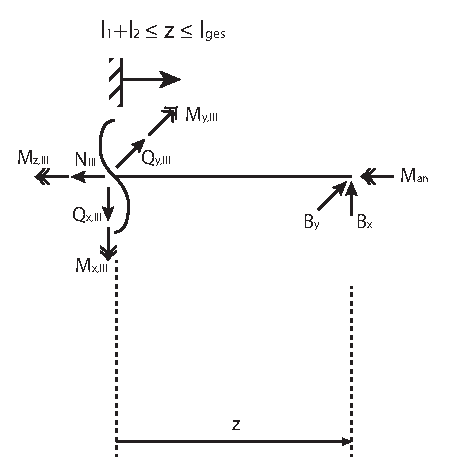
\includegraphics{figures/Bereich_3}
\end{center}
	\begin{align*}
        \sum F_x &\overset{!}{=} 0 = B_x - Q_{x,\mathrm{III}} 
				\implies  Q_{x,\mathrm{III}} = B_x = 180,11 \text { N}\\ \\
        \sum F_y &\overset{!}{=} 0 =- B_y - Q_{y,\mathrm{III}} 
				\implies Q_{y,\mathrm{III}} = -B_y = -560,8 \text{ N}\\ \\
		\sum F_z &\overset{!}{=} 0 = -N_{\mathrm{III}} -F_K
				\implies N_{\mathrm{III}} = -F_K = -2318,49 \text{ N} \\ \\
        \sum M\textsubscript{x}\textsuperscript{(P)} &\overset{!}{=} 0 =- M_{x,\mathrm{III}} +(l_3-z_3) \x B_y \\
				&\implies M_{x,\mathrm{III}} = (l_3-z_3) \x B_y = 205,5 \text{ Nm} -560,8 \text{ N} \x z_3 \\ \\
		\sum M\textsubscript{y}\textsuperscript{(P)} &\overset{!}{=} 0 =- M_{y,\mathrm{III}} + B_x \x (l_3-z_3) \\
				&\implies M_{y,\mathrm{III}} = (l_3 -z_3) \x B_x =66 \text{ Nm} -180,11 \text{ N} \x z_3\\ \\
		\sum M\textsubscript{z}\textsuperscript{(P)} &\overset{!}{=} 0 = - M_{z,\mathrm{III}} - M\textsubscript{an}
				\implies  M_{z,\mathrm{III}} = -M\textsubscript{an} = -60,17 \text{ N}\\
	\end{align*}
\end{enumerate}
\newpage
\textbf{Eckwerte:}\\ \\
Bereich i)
\begin{align*}
	N_{\mathrm{I}} (0) &= N_{\mathrm{I}} (l_1) = -2078,59 \text{ N}\\
	Q_{x,\mathrm{I}} (0) &= Q_{x,\mathrm{I}} (l_1) = -145,44\text{ N}\\
	Q_{y,\mathrm{I}} (0) &= Q_{y,\mathrm{I}} (l_1) = 548,63\text{ N}\\
	M_{x,\mathrm{I}} (0) &=  0\text{ Nm} & M_{x,\mathrm{I}} (l_1) &= 224,39\text{ Nm}\\
	M_{y,\mathrm{I}} (0) &=  0\text{ Nm} & M_{y,\mathrm{I}} (l_1) &= 59,48\text{ Nm}\\
	M_{z,\mathrm{I}} (0) &= M_{z,\mathrm{I}} (l_1) = 0\text{ Nm}\\
\end{align*}
Bereich ii)
\begin{align*}
	N_{\mathrm{II}} (0) &= N_{\mathrm{II}} (l_2) = -2318,49 \text{ N}\\
	Q_{x,\mathrm{II}} (0) &= Q_{x,\mathrm{II}} (l_2) = 183,18\text{ N}\\
	Q_{y,\mathrm{II}} (0) &= Q_{y,\mathrm{II}} (l_2) = -569,23\text{ N}\\
	M_{x,\mathrm{II}} (0) &= 224,39\text{ Nm} & M_{x,\mathrm{II}} (l_2) &= 189,83\text{ Nm}\\
	M_{y,\mathrm{II}} (0) &=  72,23\text{ Nm} & M_{y,\mathrm{II}} (l_2) &= 61,11\text{ Nm}\\
	M_{z,\mathrm{II}} (0) &= M_{z,\mathrm{II}} (l_2) = -59,42\text{ Nm}\\
\end{align*}
Bereich iii)
\begin{align*}
	N_{\mathrm{III}} (0) &= N_{\mathrm{III}} (l_3) = -2318,49 \text{ N}\\
	Q_{x,\mathrm{III}} (0) &= Q_{x,\mathrm{III}} (l_3) = 180,11\text{ N}\\
	Q_{y,\mathrm{III}} (0) &= Q_{y,\mathrm{III}} (l_3) = -560,8\text{ N}\\
	M_{x,\mathrm{III}} (0) &= 205,5\text{ Nm} & M_{x,\mathrm{III}} (l_3) &= 0\text{ Nm}\\
	M_{y,\mathrm{III}} (0) &=  66\text{ Nm} & M_{y,\mathrm{III}} (l_3) &= 0\text{ Nm}\\
	M_{z,\mathrm{III}} (0) &= M_{z,\mathrm{III}} (l_3) = -61,11\text{ Nm}\\
\end{align*}
\newpage
\section{Resultierende Momente}
\[
	|M_{b,res}(z)| = \sqrt{\left( M_{by}(z) \right)^2 + \left( M_{bx}(z) \right)^2 }
\]
Bereich i)
\begin{align*}
	&|M_{b,res}(z=0)| = 0 \text{ Nm} \\
	&|M_{b,res}(z=l_1)| = 232,14 \text{ Nm} \\
\end{align*}
Bereich ii)
\begin{align*}
	&|M_{b,res}(z=l_1)| = 235,73 \text{ Nm} \\
	&|M_{b,res}(z=l_1+l_2)| = 199,42 \text{ Nm} \\
\end{align*}
Bereich iii)
\begin{align*}
	&|M_{b,res}(z=l_1+l_2)| = 199,42 \text{ Nm} \\
	&|M_{b,res}(z=l_{ges})| = 0 \text{ Nm} \\
\end{align*}
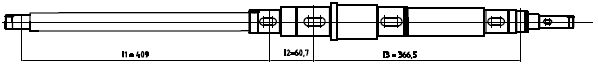
\includegraphics[width=\textwidth,keepaspectratio]{figures/Welle1klein.png}